\documentclass[]{article}
\usepackage{authblk}
\usepackage{graphicx}
\usepackage{cite}
\usepackage{url}
\usepackage{float}
\usepackage{subfigure}
\usepackage{amsfonts,amssymb}
\usepackage{amsmath}
\usepackage{amsthm}
\usepackage{float}

%opening
\title{Neural-based epidemics prediction of COVID-19}
\author{Dexin Li 201905130191}
\author{Yinchen Liu 201900130078}
\affil[1]{Shandong University\\School of Computer Science}

\begin{document}
	

\maketitle

\begin{abstract}
\par
The 2019-nCoV epidemic has totally changed our life. In order to limit its spread, every country has taken measures to limit public contacts and attempt to cure patients. Many of us are interested in how does the strict controls impact in the epidemic, and how soon will the society go back to normal. Instead of using heavy neural network structures or huge datasets, We propose a novel data pre-processing method, which help to get rid of some disadvantages of RNNs. We integrated epidemic data in China and deep-LSTMs to predict the data in worldwide. Our results show that the epidemic will probably converge by Aug.13, 2020.
\end{abstract}

\section{Introduction}
\par
The corona-virus is one of the most contagious virus to hit our society. In December 2019, the outbreak of corona-virus occurred in Hubei Province, China. This epidemic explodes out rapidly. In January 21st, 2020, this virus has caused 262 infections. By May 5th, the confirmed data has risen to 3659271, surpassing the 2003 outbreak of SARS. In order to control the status, governments had carried out policies to limit physical contacts. Everybody wants to know how soon will the epidemic end. However, the policies are so complicated and the execution of people are so different, making the estimation difficult.
\par
Time had witnessed the development of Artificial Intelligence(AI). Nanshan Zhong et.al\cite{JTD36385} had modified the original SEIR model to emphasis the importance of dynamic Susceptible and Exposed population, which is state of the art. Including AI, Nanshan Zhong et.al also applied LSTM to the epidemic prediction. Deep Learning method had been used to predict various type of epidemic\cite{Liu2017Predicting}. However, the principle of deep learning is hard to parse. Further more, deep learning takes a strict requirement of dataset, while epidemic data is full of noise and the quantity is not huge enough for deep network. Therefore, we used LSTM only for curve pattern exaction, just like Language Model(LM) in Natural Language Processing. We used a novel differential method to transfer curve prediction to LM. The training data comes from 2019 nCoV data in China, which turns out to be nearly convergent.

\section{Data Smoothing}
\subsection{Data Source}
\paragraph{}
We used
confirmed, recovered and death data of COVID-19 in worldwide as validation data\cite{bingdata}, and COVID-19 in China as training data. This is because the epidemic in China had almost come to an end. We also need data of SARS\cite{whodata} for comparation.
\subsection{Data Processing}
\paragraph{}
This part is to describe what data structure we use for data interaction.
After loading data, the function will return a two-dimentional-array.
Each one-dimensional-array stores data for one country, whose element 
is an "Data" object represents the data of that country one day. 
So the whole Data structure is like this:
\begin{figure}[H]
    \centering
    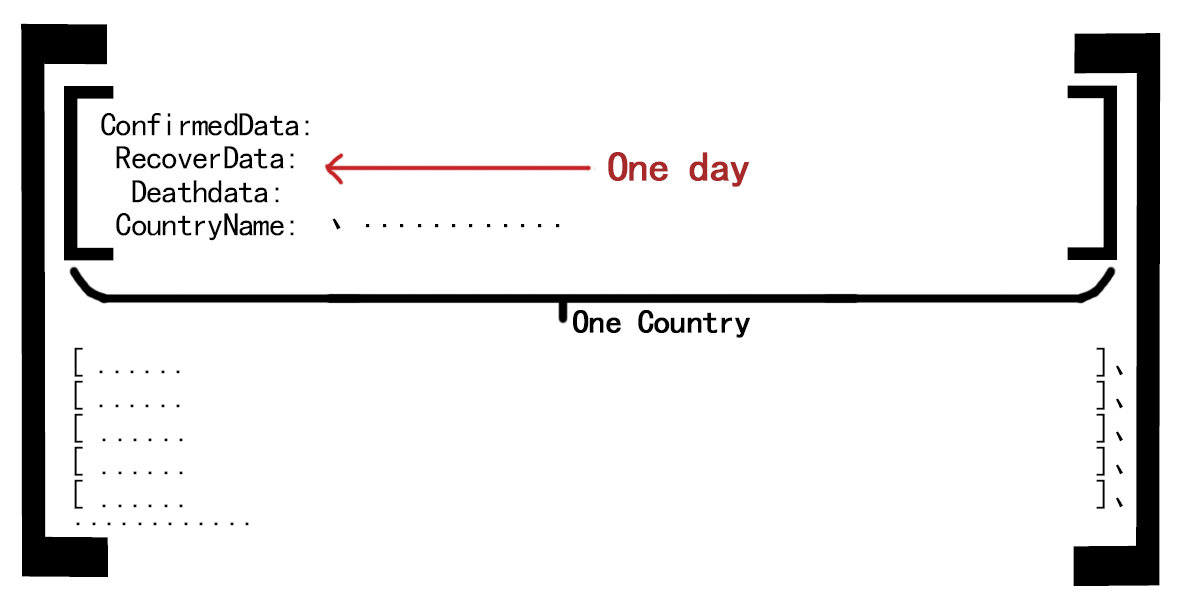
\includegraphics[width = 0.6\textwidth]{Data_Structure.png}
    \caption{Data Structure}
\end{figure}
\subsection{Curve Smoothing}
\paragraph{}
The machine learning model requires high smoothness of the input data, 
and the curve formed by the original data does not meet the requirements, 
so curve smoothing is required.
We tried three methods, polynomial fitting, cubic spline interpolation,
and B-Spline.
\par
After testing, we discoverd using the first two methords to process
the data will produce large false oscillations.
\begin{figure}[H]
    \centering
    \subfigure[False oscillations of polyfit]{
        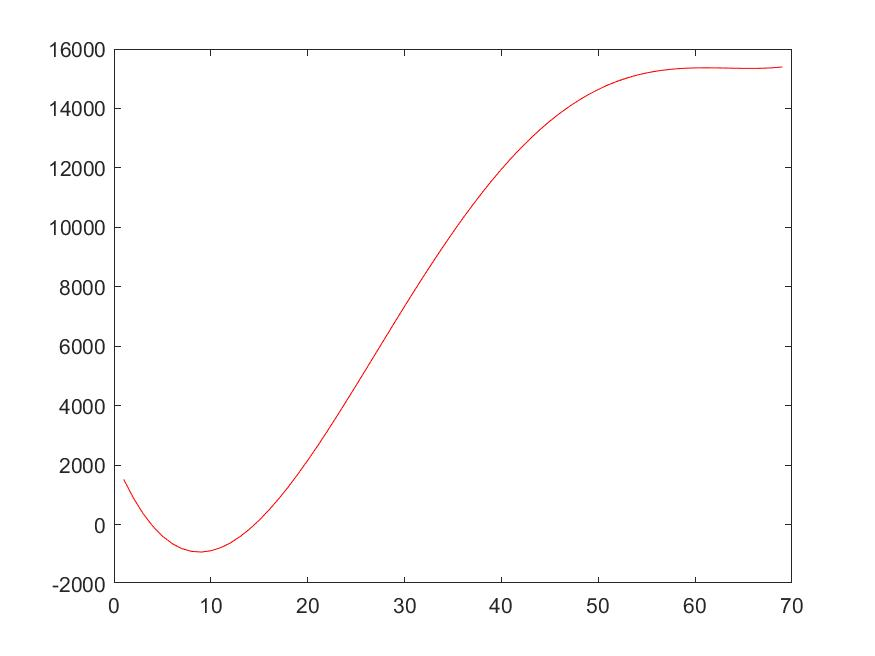
\includegraphics[width = 0.4\textwidth]{Austria.jpg}
    }
    \subfigure[False oscillations of cubic spline interpolation]{
        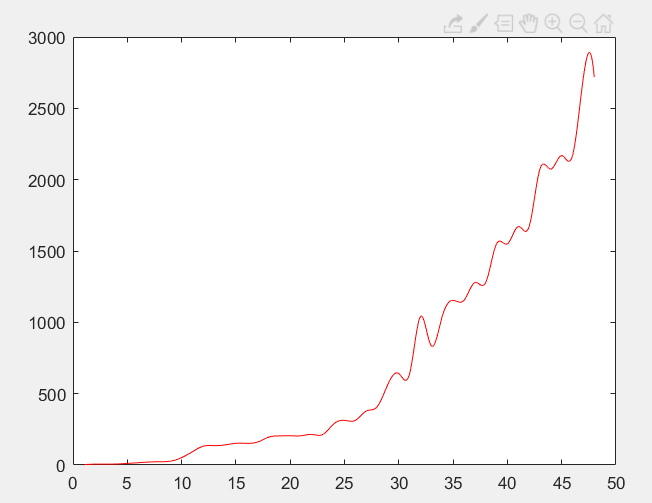
\includegraphics[width = 0.4\textwidth]{Chana.png}
	}
	\caption{False oscillations}
\end{figure}
\par
And finally decided to use the second-order B-Spline.
Using this method, 
while ensuring that the result is relatively smooth, 
the result is highly compliant with the original data 
and basically does not produce false oscillations.
\begin{figure}[H]
    \centering
    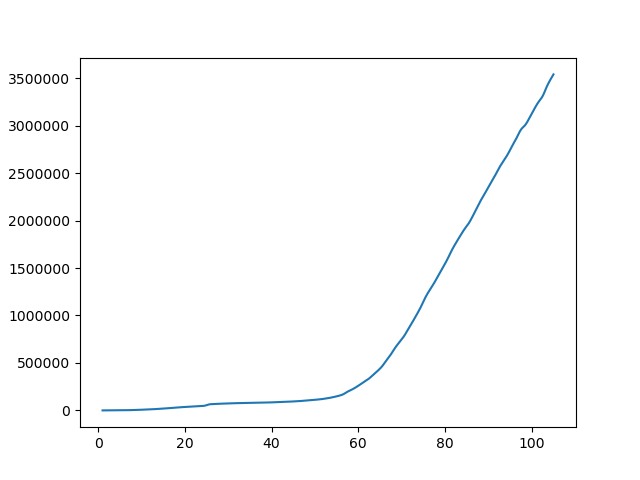
\includegraphics[width = 0.75\textwidth]{Worldwide.png}
    \caption{Worldwide data after smoothing}
\end{figure}

\section{Preliminaries}
The LSTM model is a type of RNN model which used forget gate and $\tanh$ layer to maintain its long-time memory. Deep LSTM turns out to be not interpretive. Generally, LSTM receives a series of input:
\begin{center}
\begin{math}
I = \left\{
v_1, v_2, \cdots, v_n
\right\}
\end{math}
\end{center}
, where $v_i$ is a vector of a definite dimension $m$. An LSTM can be regarded a function defined in $\mathbb{R}^{m \times n}\rightarrow \mathbb{R}$.
\par
Training is a process that fit the function into a dataset, so that the neural output of the input in dataset fits the dataset. The neural network will return an interpolation if the input does not come from the original dataset.

\section{Mechanism}
\par
The original LSTM, which receives a huge raw dataset as training data(i.e. epidemic data of the past 20 years), turns out to be not such reasonable. The 2019 nCoV is more contagious than any epidemic before, and no interpolation between training set fits the status.
\par
We notice that the infected curve goes to a definite shape. It is always an exponential curve when the virus or bacterial start to spread. As government notices the epidemic, the derivative of the curve starts to go down. In the end, the infected are controlled and the curve converges. It is the shape that determines the trend. Therefore, we only need to predict the curvature of the curve. However, the actual data is dispersed, which made the curvature impossible to compute. We used a substitute function for curvature. Define that:
\begin{center}
	\begin{math}
	C^{\prime}(x, y) = \tfrac{ \dfrac{\mathrm{d}^2 y}{\mathrm{d}x^2} } { \dfrac{\mathrm{d} y}{\mathrm{d}x} }
	, x, y\in \mathbb{R}
	\end{math}
\end{center}
Its dispersed form is:
\begin{center}
	\begin{math}
		\begin{aligned}
	C(x, y) &= \dfrac{ \dfrac{(y_{x+1} - y_{x}) - (y_{x} - y_{x-1}) }{2} } { \dfrac{y_{x+1} - y_{x-1}}{2} }
	\\
	&=\dfrac{ (y_{x+1} - 2y_{x} + y_{x-1}) } { y_{x+1} - y_{x-1} }
	,\\ x > 1, y \in \mathbb{R}
		\end{aligned}
	\end{math}
\end{center}
This function uniquely determines a shape of curve. Formally, the shapes of two number sequence $\phi_x, \theta_x$ are equivalent, when
\begin{center}
	\begin{math}
	\dfrac{\phi_x - \phi_{x-1}}{\theta_x - \theta_{x-1}} = \lambda
	\end{math}
\end{center}
, where $\lambda$ is a constant.
\newtheorem*{Theorem Unique}{Theorem 1}
\begin{Theorem Unique}
Given a series of rational $\{ A_i | i \leq n, i \in \mathbb{N}, n > 1 \}$, $C(x)$ determines a unique shape of number sequence.
\end{Theorem Unique}
\begin{proof}
Sufficiency: Obviously, We can give the $A_{n+1}$ by:
\begin{center}
	\begin{math}
	A_{n+1} = A_{n-1}C(n) - 4A_n + 2A_{n-1}
	\end{math}
\end{center}
Necessity: Suppose there are two different $\phi_{n}$ and $\theta_{n}$, if:
\begin{center}
	\begin{math}
		\begin{aligned}
	\dfrac{\phi_x - \phi_{x-1}}{\theta_x - \theta_{x-1}} &= \lambda, 
	\\
	\dfrac{\phi_{x+1} - \phi_{x}}{\theta_{x+1} - \theta_{x}} &= \lambda
		\end{aligned}
	\end{math}
\end{center}
, there is:
\begin{center}
	\begin{math}
		\begin{aligned}
	C(x, \phi)&=
	\dfrac{ (\phi_{x+1} - \phi_{x}) - (\phi_{x} -  \phi_{x-1}) } { (\phi_{x+1} - \phi_{x}) + (\phi_{x} - \phi_{x-1}) }
	\\
	&= 	\dfrac{ \lambda(\theta_{x+1} - \theta_{x}) - \lambda(\theta_x - \theta_{x-1}) } { \lambda(\theta_{x+1} - \theta_x) + \lambda(\theta_x - \theta_{x-1}) }
	\\
	&= C(x, \theta)
		\end{aligned}
	\end{math}
\end{center}
\end{proof}
\par
An LSTM\cite{HochSchm97} fetches out sequential features to predict a next data. Denote the LSTM units $net^{i}$ receive a series of time-based input $A_{i}$, where $A^{tr}_{i}$ stands for training data, and $A^{in}_{i}$ stands for validation data. The expected output is denoted by $net^{out}$. A converged model should satisfy:
\begin{center}
	\begin{gather}
		\exists A^{tr_1}, A^{tr_2} \in A^{tr}, s.t.\\
		A^{in}_{i} \leqslant net^{out}(A^{tr_1})\\
		A^{in}_{i} \geqslant net^{out}(A^{tr_2})
	\end{gather}
\end{center}
It turns out that the raw epidemic data does not mean to be available in legacy LSTM, while the preprocessed data fortunately satisfies the condition.

\section{Rationality}
\par
A question is, why do we use the shape to determine a curve of epidemic? Does it fit the reality? In order to reveal its rationality, look at the two figures.

\begin{figure}[H]
	\centering
	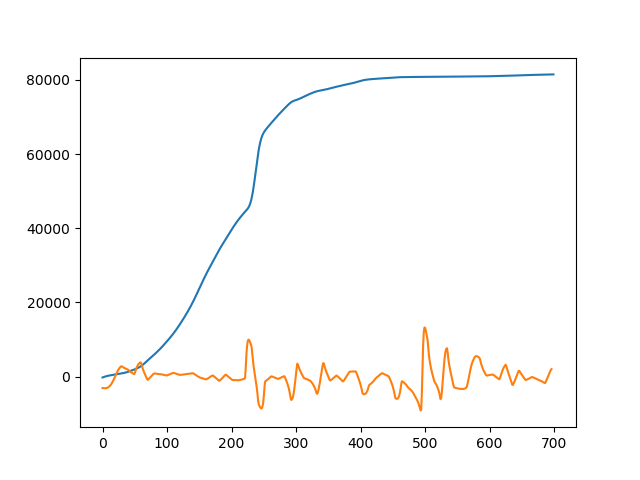
\includegraphics[width=0.7\linewidth]{Figure_nCoV_China}
	\caption{nCoV\_China}
	\label{fig:nCoV_China}
\end{figure}
\begin{figure}[H]
	\centering
	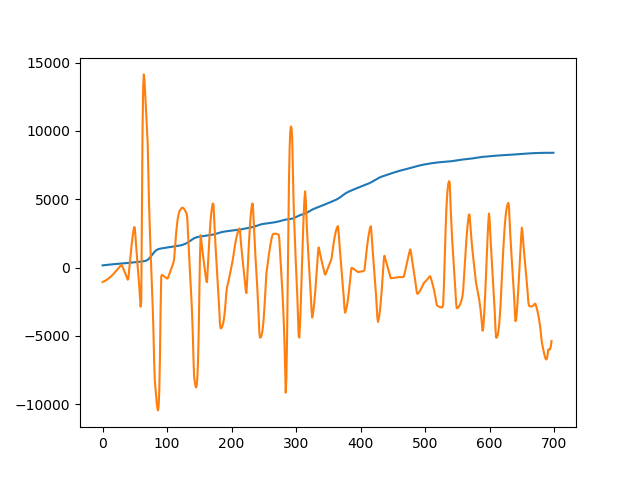
\includegraphics[width=0.7\linewidth]{Figure_SARS}
	\caption{SARS}
	\label{fig:SARS}
\end{figure}
\par
The orange curve shows $C(x, f)$, while the blue curve shows $f(x)$(notice that the curve has been smoothed and the $x$ domain has been scaled to 10 times).
\par
Notice that the $C(x, f)$ is basically an oscillation function. With the ending of epidemic comes, the vibration frequency and the amplitude are similar.

\section{Prediction}
Figure 5 shows the model prediction inputted with day $\left[ 50, 100 \right)$, while Figure 6 shows another prediction inputted with day $\left[ 20, 70 \right)$. The difference between the two figures reveals the different policies between worldwide and China.
\begin{figure}[H]
	\centering
	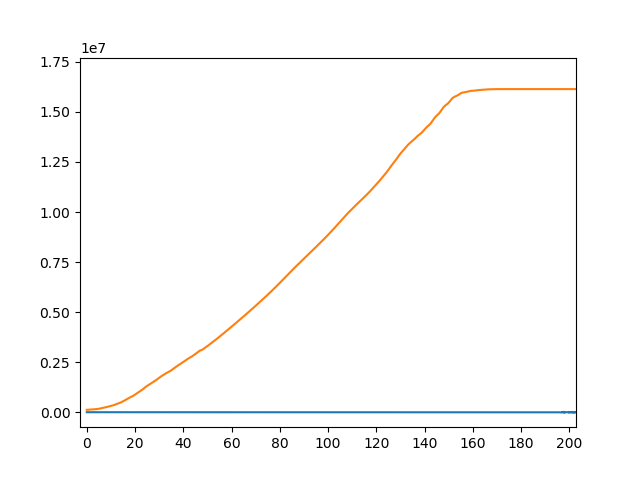
\includegraphics[width=0.7\linewidth]{Figure_1}
	\caption{$[50, 100)$}
	\label{fig:figure1}
\end{figure}
\begin{figure}[H]
	\centering
	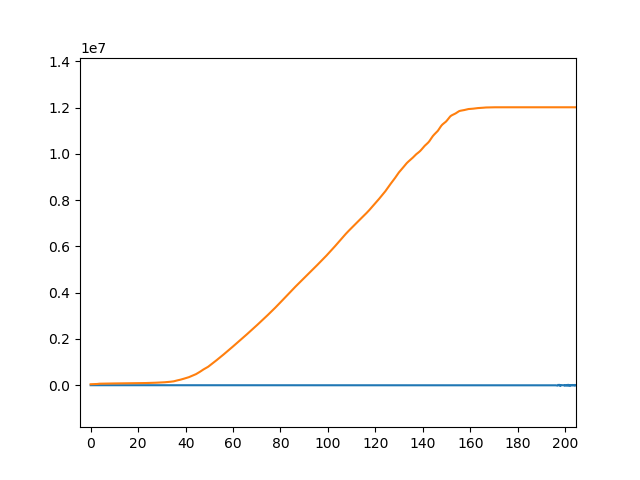
\includegraphics[width=0.7\linewidth]{Figure_2}
	\caption{$[20, 70)$}
	\label{fig:figure2}
\end{figure}

\section{Prospect}
\subsection{Epidemic curve under different policies}
\paragraph{}
The epidemic has been raging for months. Here are the predictions for the United Kingdom and Brazil.
\begin{figure}[H]
	\centering
	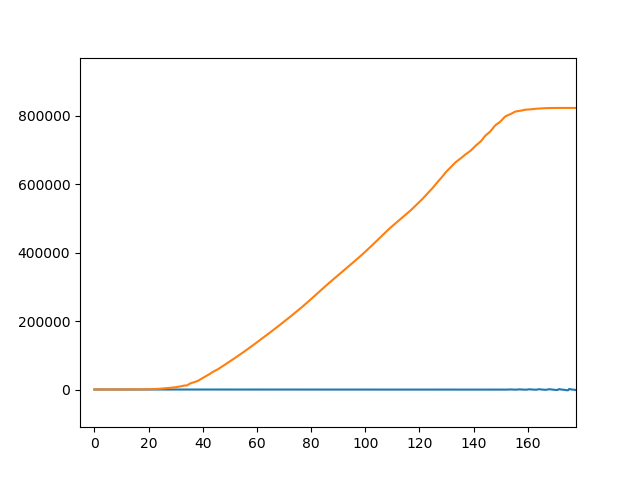
\includegraphics[width=0.7\linewidth]{Figure_England}
	\caption{The United Kingdom}
	\label{fig:figure3}
\end{figure}
\begin{figure}[H]
	\centering
	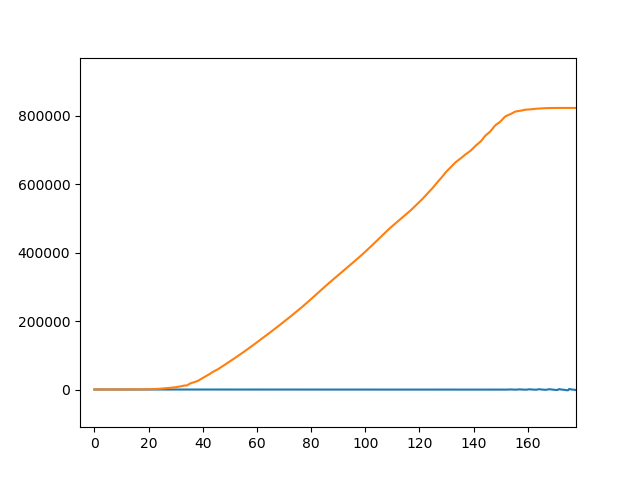
\includegraphics[width=0.7\linewidth]{Figure_England}
	\caption{Brazil}
	\label{fig:figure4}
\end{figure}
The variants in epidemic predictions is countless. The most influential one is the policies. The United Kingdom turns out to rely on Herd immunity to control the epidemic, which sacrifices too many infected. By contrast, China government has carried out effective policies, coordinated with people's execution, making the epidemic get efficacious control.
\par
The classic SIR model\cite{kermack1927a}, considered three compartments: susceptible, $S(t)$; infected, $I(t)$; removed, $R(t)$, where $t$ stands for the time. 
\begin{center}
\begin{gather}
N = S(t) + I(t) + R(t)\\
\frac{dS}{dt} = -\frac{\beta SI}{N}\\
\frac{dI}{dt} = \frac{\beta SI}{N} - \gamma I
\frac{dR}{dt} = \gamma I
\end{gather}
\end{center}
\par
It is assumed that each person has equal possibility to be infected by a suspected each time. Thus, the infecting rate can be considered as a constant $\beta$, and radius as $\gamma$. As if we take measures to avoid being infected, such as wearing a mask, or avoiding people, both $\beta$ and $\gamma$ would be lowered. The epidemic would be controlled when it is in infancy. However, if $\beta$ or $\gamma$ can not be controlled, the exponential explosion will cause a disaster.
\par
The explosion have been catching the governments' attention, and the infectious status have been cutting down.

\subsection{Number of deaths in Brazil}
\paragraph{}
We also made predictions on the number of deaths in Brazil. Accoding to the prediction above, we discoverd that the confirmed number of
Brazil wiil peak around day 150, and the death toll of Brazil wiil reach about eighty thouthand. The curve is as follow. 
\begin{figure}[H]
	\centering
	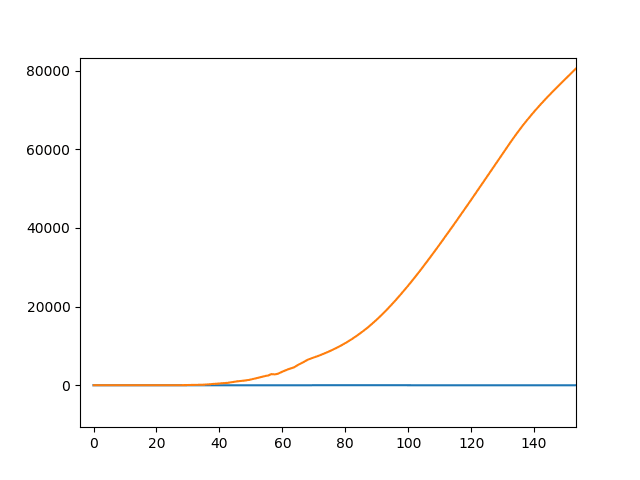
\includegraphics[width=0.7\textwidth]{Death_Brazil.png}
	\caption{Number of deaths in Brazil}
\end{figure}
And the number of deaths worldwide will reach about a million by then.
\begin{figure}[H]
	\centering
	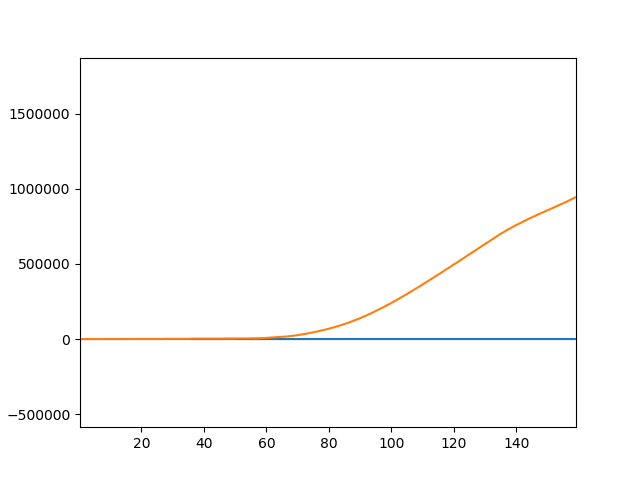
\includegraphics[width=0.7\textwidth]{Death_Worldwide.png}
	\caption{Number of deaths worldwide}
\end{figure}
\subsection{Influence of medical resources}
\paragraph{}
For the most severely affected cities, we did research on WuHan. Here is the confirmed of WuHan in February 2020.
\begin{figure}[H]
	\centering
	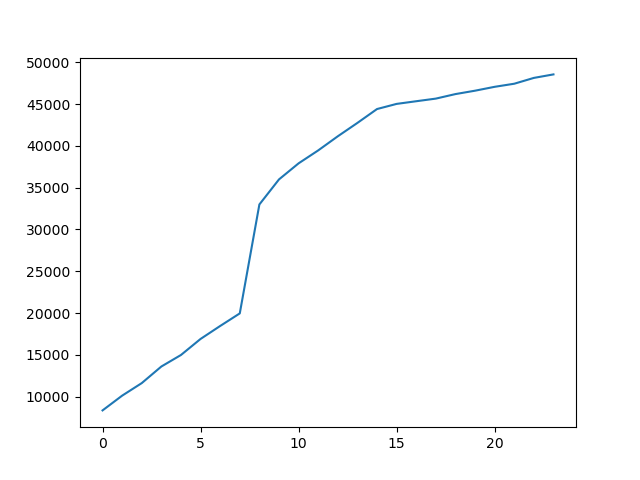
\includegraphics[width=0.7\textwidth]{Figure_WuHan.png}
	\caption{WuHan}
\end{figure}
From the figure we noticed that the confirmed number is increased very fast at the beginning, and slowed down at mid-February, 
when several mobile cabin hospitals were put into use.
\par
The conclusion is very clear : the best way to slow down the spread of the virus is centralized isolation. Cities should 
establish a system to isolating infected people centrally when facing epidemic.If so, the pressure on the hospital will be greatly relieved, community and family infections can also be reduced.
\subsection{Economic impact}
\paragraph{}
The COVID-19 hit the economy hard. Accoding to the data provided by Nation Bureau of Statistics, the total tetail sales of consumer goods fell 15.8 percent and 7.5 percent year-on-year in March and April, respectively. 
\begin{figure}[H]
	\centering
	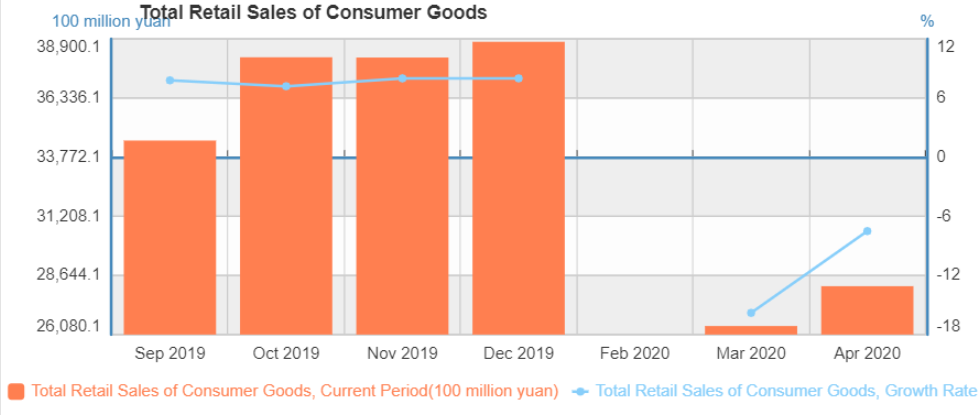
\includegraphics[width=0.7\textwidth]{Eco_2020.png}
	\caption{Total Retail Sales of Consumer Goods}
	\cite{nbsdata}
\end{figure}
\par
Looking back on 2003, the situation is very similar. The outbreak of SARS slowed down the growth rate of retail sales of consumer goods in March, April and May 2003,  and also greatly reduced the growth rate of it in 2003 the whole year.
\begin{figure}[H]
    \centering
    \subfigure[Influence in 2003]{
		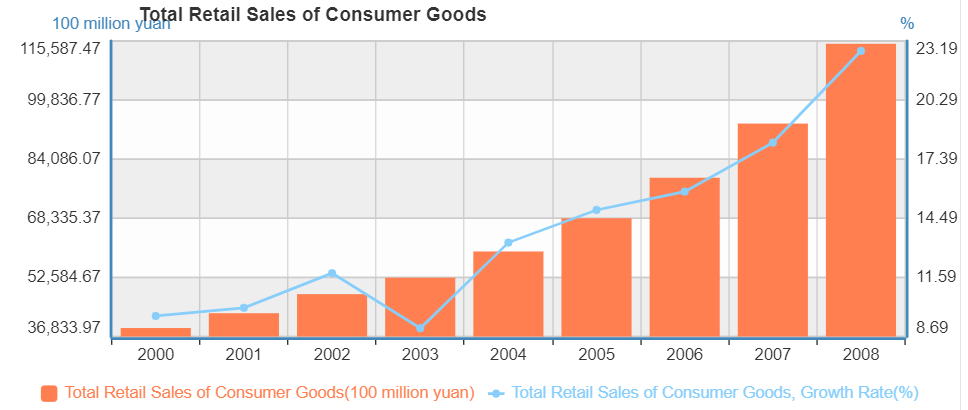
\includegraphics[width = 0.4\textwidth]{Eco_2000_2010.png}
    }
    \subfigure[Influence in 2003/5]{
		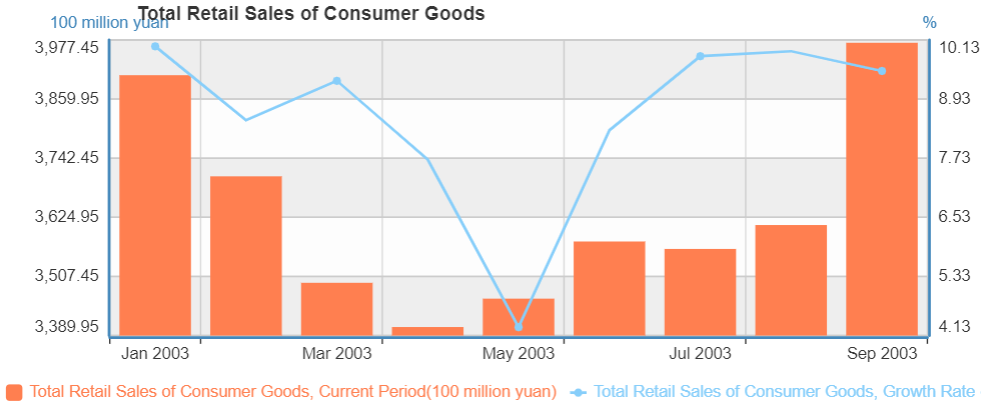
\includegraphics[width = 0.4\textwidth]{Eco_200305.png}
	}
	\caption{SARS's influence}
	\cite{nbsdata}
\end{figure}
\par
Although COVID-19 has a greater impact on the economy in the short term, observe the impact of SARS, we can find that the epidemic has little effect on the overall economic trend, so this time, we believe that the total retail sales of consumer goods this year may be lower than last year, but the overall stable situation will not change.
\bibliographystyle{plain}

\bibliography{ref}
\end{document}
